%LaTeX Example file 6

%figures, floats, and putting images in from outside

\documentclass[12pt, letterpaper]{article}

\usepackage{graphicx}
\usepackage[letterpaper, margin=1in]{geometry}


\title{Figures, Floats, and Inserting Images}
\author{Maurice Moss\\{\tt it@reynholm.co.uk}}

\begin{document}
	
	\maketitle


	\section{Inserting Images}

	\begin{figure}[htp]
		\centering
		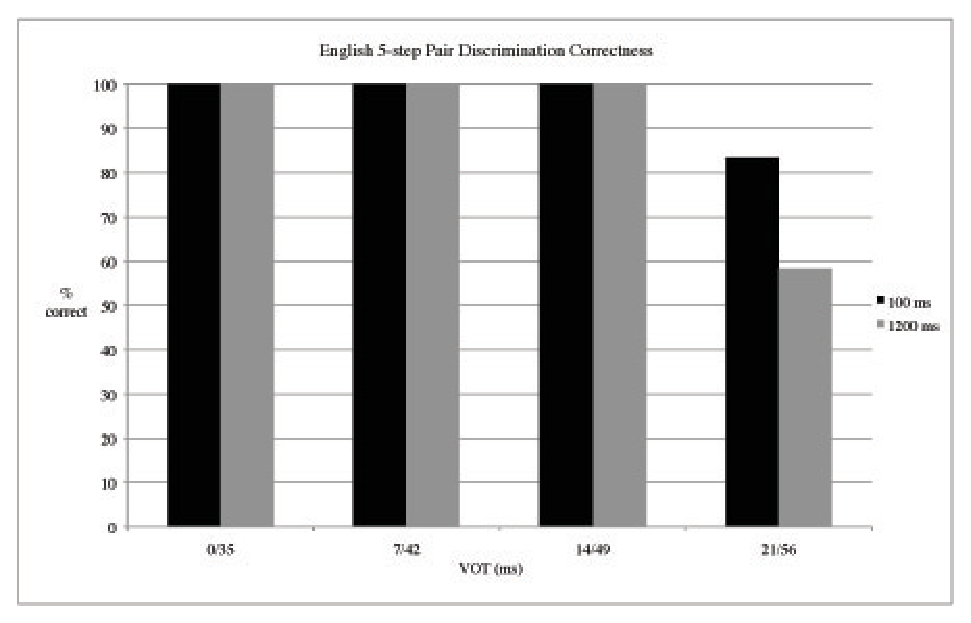
\includegraphics{english5stepcorrect}
		\caption{\% of correct responses for 5-Step Pairs in Experiments 3 and 4}
		\label{fig:english5stepcorrect}
	\end{figure}

	\begin{figure}[p]
		\centering
		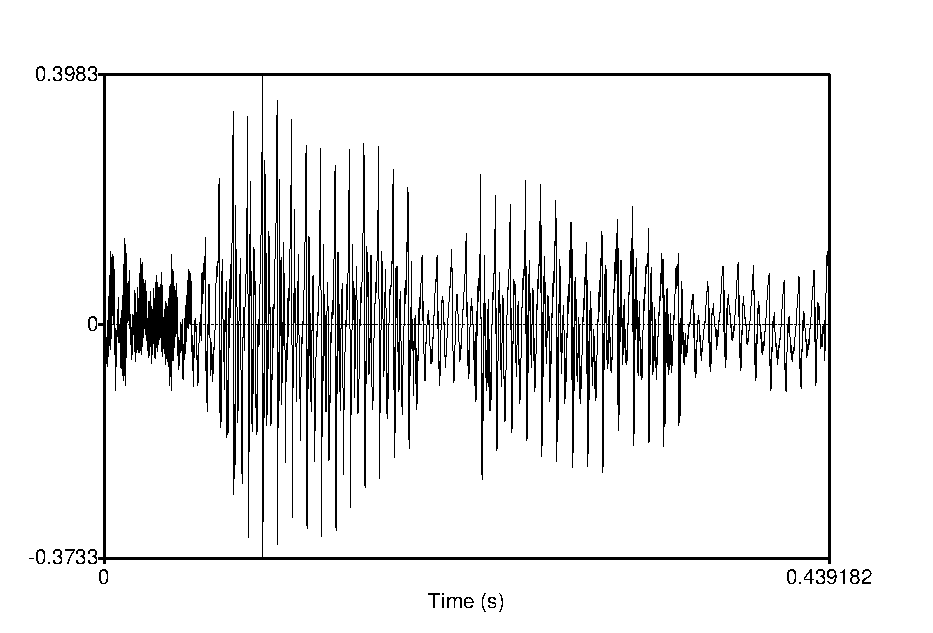
\includegraphics{waveform}
		\caption{Waveform of RB-normal-4}
		\label{fig:waveform}
	\end{figure}

	And as you can imagine, we can refer to the figures with labels, as in \ref{fig:waveform}.

	%clearpage
	\section{Other Floats and Figures}

	\begin{table}[ht]
		\caption{Name Initial Syllable Strength by Token}
		\label{tbl:strength}
		\begin{center}
			\begin{tabular}{c|ccccccc}
				\hline
				\textbf{Token:}&\multicolumn{2}{c}{1}&\multicolumn{2}{c}{2}&\multicolumn{2}{c}{3}&4\\
				\textbf{Name:}&(a)&(b)&(a)&(b)&(a)&(b)&\\
				\hline
				\hline
				Lysander&$s$&$w$&$s$&$w$&$s$&$s$&$n$\\
				Demetrius&$w$&$s$&$w$&$s$&$s$&$s$&$n$\\
				Hermia&$s$&$w$&$s$&$w$&$w$&$w$&$n$\\
				Polly&$w$&$s$&$w$&$s$&$w$&$w$&$n$\\
				\hline
			\end{tabular}
		\end{center}
	\end{table}

\end{document}